
\documentclass[14pt]{memoir}


% Lorem Ipsum Text
\usepackage{lipsum}

% Section and Figure Numbering
\renewcommand\thesection{\arabic{section}}
\usepackage{chngcntr}
\counterwithout{figure}{chapter}

% Referencing Commands
\newcommand{\refsec}[1]{\hyperref[sec:#1]{Section~\ref{sec:#1}}}
\newcommand{\reffig}[1]{\hyperref[fig:#1]{Figure~\ref{fig:#1}}}

%TiKz
\usepackage{tikz}
\usetikzlibrary{arrows}
\usetikzlibrary{shapes}

% CMU sans serif font.
\usepackage[T1]{fontenc}
\renewcommand*\familydefault{\sfdefault}

% Hyperlinks
\usepackage{hyperref}
\hypersetup{
    colorlinks=true,       % false: boxed links; true: colored links
    linkcolor=black,          % color of internal links (change box color with linkbordercolor)
    citecolor=black,        % color of links to bibliography
    filecolor=blue,      % color of file links
    urlcolor=blue           % color of external links
}

% APA 6 citation and bibliography style % Note: Must be loaded after hyperref
\usepackage{apacite} 

% Abbreviations
\usepackage{glossaries}
\makeglossaries

\newacronym{pisa}{PISA}{Programme for International Student Assessment}
\newacronym{oecd}{OECD}{Organisation for Economic Co-operation and Development}
\newacronym{stem}{STEM}{Science, Technology, Engineering and Mathematics}
\newacronym{fmri}{fMRI}{functional magnetic resonance imaging}
\newacronym{naplan}{NAPLAN}{National Assessment Program --- Literacy and Numeracy}
\newacronym{mars}{MARS}{Maths Anxiety Rating Scale}
\newacronym{mas-r}{MAS-R}{Maths Anxiety Scale --- Revised}
\newacronym{ptsd}{PTSD}{Post-Traumatic Stress Disorder}



\title{Maths Anxiety: Theory to Practice}
\author{Lyron Winderbaum}



\begin{document}



\maketitle



\begin{abstract}

\lipsum[1-2]

\end{abstract}
% 100-150 words


\glsresetall
\section{Literature Review (/1100 words)}

\subsection*{Prevalence}

Maths anxiety is hugely prevalent, and consequently the literature describing research around it is extensive. The \citeA{PISA2013} 2012 \gls{pisa} report states that across \gls{oecd} countries, over 30\% of 15 year old students ``get very nervous doing mathematics problems'', and over 60\% of students ``worry about getting poor grades in mathematics''. 
% ``Across OECD countries, 59\% of students reported that they often worry that it will be difficult for them in mathematics classes; 33\% reported that they get very tense when they have to do mathematics homework; 31\% that they get very nervous doing mathematics problems; 30\% that they feel helpless when doing a mathematics problem, and 61\% that they worry about getting poor grades in mathematics''.  

\subsection*{Why is Maths Anxiety Important?}

It is my view that as teachers our foremost concern should be for the wellbeing of our students. \citeA{Lyons2012pain} used \gls{fmri} to demonstrate that students categorised as having a high level of maths anxiety will often experience the anticipation of a maths task as visceral pain. Moral imperative (and ethical duty of care) requires us to take every step possible to protect our students from such an experience.

Beyond the clear and overwhelming wellbeing concerns, it is also important to recognise the connection between maths anxiety and performance, and the complex web of stakeholders surrounding a students academic success in maths. \citeA{Foley2017} discuss the negative correlation between maths anxiety and performance shown in the 2012 \gls{pisa} \cite{PISA2013} report, and also note the rising demand for \gls{stem} professionals worldwide. It has been shown that when a student has low self-concept (correlated with high maths anxiety), they will tend not to enroll in maths beyond the minimum requirements for graduation \cite{Ashcraft2007book}. Beyond highschool graduation, it has been shown that students affect towards maths can predict their university major \cite{LeFevre1992}. So although many governments and industries around the world are recognising their need for more mathematics-qualified graduates, addressing maths anxiety may be a key piece to the puzzle of filling this demand.

%Maths performance, and hence the maths anxiety-performance link is important to many other stakeholders as well. Parents who want their children to acheive academic success in maths, students themselves feeding back into their own self-concept and self-efficacy, and schools which are often ranked and funded based on their students academic acheivement, with maths being a recurring problem subject for many schools. In an Australian context one important way in which schools and ranked and funded is through \gls{naplan}. Ultimately it is difficult to seperate any maths anxiety research from the concept of maths performance, for better or for worse.
%
%So although I think students wellbeing should be reason enough for maths anxiety to be important, there are many reasons beyond their wellbeing alone that make it a critical area to address.

\subsection*{History of Maths Anxiety as a Distinct Phenomena to General Anxiety}

The existence of maths anxiety as ``emotional disturbances in the presence of mathematics'' has been noted as early as the 1950's, \citeA{Dreger1957} even postulated that what he tentatively designated ``Number Anxiety'' and later became to be known as Maths Anxiety could be a distinct syndrome from general anxiety. Later the landmark meta-study of \citeA{Hembree1990} supported this hypothesis, showing a correlation of only $0.38$ between maths anxiety and general anxiety. In more recent times, this hypothesis has also been confirmed by \citeA{Young2012} using \gls{fmri} to show that the brain activity in a person experiencing maths anxiety is measurably distinct from that in a person suffering general anxiety. These later studies including the meta-analysis of \citeA{Hembree1990} but also later the work of \citeA{Kazelskis2000} and others further delineated maths anxiety from test anxiety, and this work continued until today it is quite well accepted that these anxieties although they share some overlap, are meaningfully distinct constructs. For more on the history of maths anxiety, \citeA{Pellicioni2016} offers a more detailed review.

\subsection*{History of Instruments for Measuring Maths Anxiety}

Significant work has been done over the years to develop psychometrics to measure maths anxiety, almost exclusively consisting of self-reporting surveys (with the exception of some more modern \gls{fmri} work, such as that of \citeA{Lyons2012}). One of the earliest instruments for measuring maths anxiety was the \gls{mars} 98-item 5-point Likert scale of \citeA{Richardson1972}. Since then, many different groups have split off and created various revised versions of a number of offshoots of this original idea, but all rely on a self-reporting survey. An example of one of the more recently developed scales is the \gls{mas-r} of \citeA{Bai2009}, which they later did some work to demonstrate was very reproducible \cite{Bai2011}.

\subsection*{Current Theories on the Maths Anxiety-Performance Link}.

It is difficult to separate the study of maths anxiety itself from research about the maths anxiety-performance link, and so most maths anxiety research, with the possible exception of some of the recent \gls{fmri} work such as \citeA{Young2012} and \citeA{Lyons2012pain}, is actually research on the maths anxiety-performance link. As summarised by \citeA{Ramirez2018}, there are two broad modes of thought in terms of explaining the maths anxiety-performance link. I will adopt the terminology of \citeA{Ramirez2018} for these: the ``Disruption Account'' and the ``Reduced Competency Account''. \citeA{Ramirez2018} make a convincing argument that although these two modes of thought might seem to compete at first glance, they are in fact not mutually exclusive and are actually compatible with each other. \citeA{Ramirez2018} suggests a third ``Interpretation Account'' which encapsulates observations made by both lines of research, see \reffig{ramirez}.

\begin{center}
\begin{figure}
\begin{center}
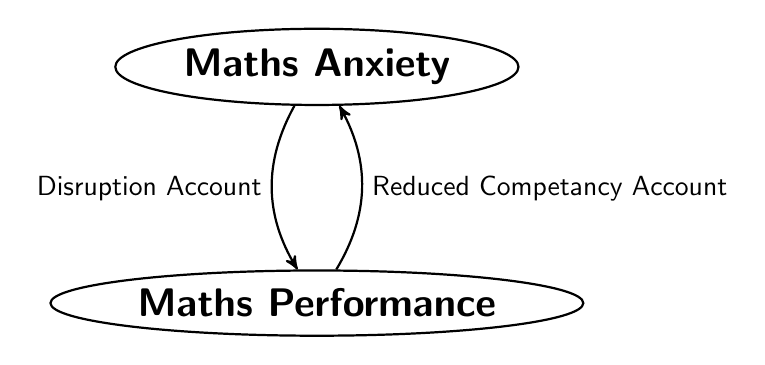
\begin{tikzpicture}[->,>=stealth',auto,node distance=3cm,thick,main node/.style={ellipse,draw,font=\sffamily\Large\bfseries}]
  	\node[main node] (a) {Maths Anxiety};
 	\node[main node] (b) [below of=a] {Maths Performance};

	\path	(a) edge[bend right] node [left] {Disruption Account} (b)
		(b) edge[bend right] node [right] {Reduced Competancy Account} (a);
\end{tikzpicture}
\end{center}
\caption{The Interpretation Account of Ramirez et al. (2018) for the maths anxiety-performance link showing how the Disruption Account and the Reduced Competency Account can be compatible.
\label{fig:ramirez}}
\end{figure}
\end{center}

The ``Disruption Account'' is currently considered as the dominant theory, seemingly spearheaded by the work of Ashcraft et al. and is based on a body of work centered around the concept of working memory \cite{Ashcraft2001, Ashcraft2007}. Specifically, the thought is that maths anxiety takes up students working memory, which prevents them from using that working memory to complete maths tasks and hence impacts performance. The ``Reduced Competency Account'', which seems to be less popular in recent times, claims that lower ability in maths leads to negative experiences associated to maths, and that these negative experiences cause maths anxiety to develop. There is also a significant body of work to support this hypothesis, including the meta-analysis of \citeA{Hembree1990} discussed above and more recent follow-up work such as the large longitudinal study of \citeA{Ma2004} which found that although past maths anxiety was correlated with future maths performance it was a small effect, while past maths performance had a strong effect on future maths anxiety.

\subsection*{Complexities in Designing and Implementing Interventions}

These large theoretical views are of course oversimplifications of what is an incredibly complex and interconnected topic. They also imply very different approaches for intervention. The ``Reduced Competency Account'' would imply interventions to boost maths performance and hence allow students to experience success in math should also help to reduce maths anxiety. The results of  \citeA{Supekar2015} seem to support this hypothesis as when students are given an intensive 8-week tutoring program to boost their maths skills, this is associated to a reduction in maths anxiety. However \citeA{Jansen2013} showed that although students attempt more problems and perform better when they are experience more success in maths, their improved performance is almost completely predicted by the number of problems they attempted, not their experience of success. To confuse things further, in the work of \citeA{Jansen2013} the improved performance did not appear to have any effect on maths anxiety, although this may be limited by the fact that it was a single time-point study. \citeA{Faust1996} demonstrated an anxiety-complexity effect which further supports the implication that scaffolding is an important component in maths anxiety interventions. \citeA{Faust1996} showed that low and high maths anxiety groups perform similarly on low complexity problems, but in high complexity problems the high anxiety groups performance is impacted.
	
On the other side of the intervention spectrum are ``Disruption Account'' motivated approaches motivated by the understanding that if students maths anxiety can be reduced, they will have increased working memory available, and their performance will improve. One fairly direct and successful attempt at this is that of \citeA{Park2014}, in which they used expressive writing exercises to help guide students self-perceived narratives about their maths experiences and thereby reduce their maths anxiety. Notably the approach of \citeA{Park2014} is in line with some successful exposure based treatments for clinical anxiety disorders including \gls{ptsd} (see \citeA{Becker2007} and \citeA{Foa2005}). Another approach that has shown success in this vein does not attempt to directly reduce the anxiety experienced, but rather reappraise it's symptoms \cite{Jamieson2016}. In this approach stress is reconceptualised as a coping tool, an evolutionary method for heightening performance in response to a challenge to be overcome, instead of a symptom of exposure to something to be feared and avoided. The work of \cite{Wang2015} shows the role of intrinsic motivation in mediating the relationship between maths anxiety and performance --- specifically that although in students with low intrinsic motivation a direct negative correlation was observed between math anxiety and performance, in high intrinsic motivation students this was not the case, instead a inverted U-shape association was observed, implying that a moderate amount of anxiety was correlated to improved performance for these students. The proposed interpretation for this more or less lies int he area of `productive struggle'. \citeA{Lin-Siegler2016} expose students in a classroom to struggles experienced by famous scientists in order to help normalise the concept of productive struggle, a concept that has also been discussed as important in the maths classroom \cite{Hiebert2007}.
 
Should write a wrap-up of the lit. review.


\section{Proposed research design/ methodology/ budget outline (/700 words)}

I propose a four-fold approach for addressing maths anxiety:

\begin{itemize}
	\item An intensive tutoring program to boost students math abilities, along the same lines as that of \citeA{Supekar2015}.
	\item Coaching around reappraisal of physiological signs of stress (increased heart rate, sweaty palms, etc.) such as that of \citeA{Jamieson2016} to interpret these signs as an evolutionary trait that increases fitness and performance in response to a challenge, instead of interpreting them as signs of danger to run from and avoid.
	\item Guided expressive writing, such as the approach of \citeA{Park2014}, based on and similar to clinical psychological therapy approaches to treating other anxieties that have been shown to be effective.
	\item Teacher coaching and visiting expert demonstrations on how to engage in ``productive struggle''.
\end{itemize}

My hypothesis is that there will be an interaction effect between these different approaches, that where one approach may fail for a particular student, a combined approach could succeed. 

To test this hypothesis we will do an initial trial, and then follow the participants longitudinally to identify potential longterm effects
caused by changed mindset towards mathematics by trajectory analysis. 

Hello




\section{Ethics Issues (/100 words)}

\section{Executive Summary (/100-150 words)}



\printglossaries

\glsresetall
\bibliographystyle{apacite}
\bibliography{citations} 

\end{document}


